\chapter{Theory} \label{ch:theory}
In this chapter some preliminary theory on 3D scanning, mathematics and computer science is presented. These notions will be applied in the following chapters.

\section{3D Scanning}
The general goal of a 3D scanning project is to create a digital representation of a physical three-dimensional object. Different methodologies exist for all sizes and types of objects. This section will give an overview of the process of 3D scanning, including the technology involved in obtaining 3D data, the operations that are performed to process it, and the final results a 3D scanning project aims to obtain.

Possibly the most simple case is to scan the surface of a single, solid object. Examples include artefacts such as the commonly used \emph{Stanford Bunny}, models of teeth or bones for manufacturing of prosthesis, small archeological artifacts, etc. The object is idealised mathematically as a single closed two-dimensional surface embedded in three-dimensional space.

To scan an object, typically 3D scanners and photogrammetry are used. Laser scanners emit light and detect the reflections from the object, in order to record a set of three-dimensional coordinates of points lying on the object's surfaces. For smaller objects, contact scanners which physically probe the object also exist. Photogrammetry consists of taking multiple photographic pictures of the object, and algorithmically recovering depth information by comparing photos from different camera poses. The scanning system can be set up such that the object and/or the scanners and cameras are rotated until the entire object is covered.

For larger of more complex objects, or for objects embedded in a more complex environment, it becomes harder to delimit the targeted content, and to filter it out from the raw scans. This is for instance the case for buildings \cite{Kers2006}, archeological sites \cite{Kein2011} \cite{Grus2012} or rock formations. It may be desirable to record specific parts of the scene at a higher resolution. Data is collected using a combination of laser scanning and photogrammetry, where the scanner is kept at a fixed position relative to the object. The result is a \emph{range image} or \emph{depth map}, a projected two-dimensional image of the object from a given view point where each pixel contains depth information.

Post-processing of the 3D scans consists in filtering the raw data and combining range images and photographs from different view points, in order to obtain a full 3D model of the entire object. This resulting 3D model is an approximation of the real object's surfaces, typically in the form of a set of unconnected points (\emph{point cloud}), or of a \emph{mesh} of vertices forming triangular faces. In some applications, such as in architecture or in retro-engineering, the goal is to obtain a CAD model, in which shapes like planes or cylinders, or more complex objects, are identified. 

In other contexts, specifically in medical imaging, the goal is not to scan surfaces, but the whole insides of an object. Here techniques such as \emph{computed tomography} and \emph{magnetic resonance imaging} are used, and a volumetric model of the object in the form of \emph{voxel data} is produced. A \emph{voxel} is the three-dimensional equivalent of a \emph{pixel}.

Other applications of laser scanning include for example meteorology, where backscatter in the atmosphere is measured, forestry, where airborne laser scanning is used to obtain a terrain height-map with multiple layers representing the ground and treetops, the scanning of astronomical objects, robotics \cite{Bibe2003} or autonomous vehicles, and more.

This paper focusses on the problem of registering different scans of parts of the same object, especially in the case where the scans have different resolutions. The scanned object is modeled to be an ensemble of continuous surfaces, and the point clouds a discrete set of points from those surfaces.


\subsection{Point cloud}
In the context of this paper, data obtained from 3D scanning is recorded in the form of a \emph{point cloud}. An unorganized point cloud is defined as a set $P = \{ (x_i, y_i, z_i) \}$ of \emph{points}, each of which have cartesian spatial coordinates defined in a coordinate system specific for this scan. Each point can be attributed with additional information, such as an RGB color, a temperature, or the normal vector of the surface at that point. Laser scanners usually record an intensity value that records the strength of the reflected light beam at that point, and possibly a confidence value indicating the correctness of the measurement.

Point clouds hold no information about the connectivity of the points that form a surface of the object. Points that are considered to be samples of a surface are called \emph{inliers}. Each inlier has a certain \emph{error} as a result of the limited precision of the scanner, and due to properties of the material. The error can be defined as the point's offset from the actual surface. Points that do not form part of the object surface are called \emph{outliers}. They may be the result of unwanted content that got scanned along with the targeted object, or any other \emph{noise} data that appears during the processing pipeline.

Representing real objects using point clouds can be considered to be a two-fold modeling of physical reality: First it is assumed that the object is a set of continuous, solid surfaces. This disregards material properties such as surface reflectance and transparency, fine-scale texture of the surface and the resulting effects on light reflection, small scale motions of the object. Within this model point attributes such as a surface normal vector and color are defined, and points get classified as inliers or outliers. Then this surfaces model is represented by means of a sparse set of points, which introduces additional considerations such as the dispersion, density and uncertainty of the points.

This notion is vague, and can be inappropriate when the real object is too complex to be modeled that way. For example for brick wall covered with climbing plants, scanned at low resolution, which are possibly in motion during the scan, there is not enough information available in the point cloud to represent the surfaces of the individual leaves. When instead considering the wall to be one plane, the vegetation gets represented as an error value in subsequent processing.


\subsection{Range image} \label{sec:range_image}
Additional information can be contained in the ordering of the points in the recorded point cloud data. Laser scanners probe their field of view by sending out rays in different directions in a well-defined order. Typically the elevation and azimuth angles are gradually incremented and reset in a line-by-line manner, forming a two-dimensional grid in the field of view. Knowing the width and height of this grid, the ordered point cloud corresponds to a \emph{range image}.

Each pixel in the range image corresponds to either a point $p_i \in P$, or an invalid point $\epsilon$, in case when no reflected ray was received in the direction the scanner was pointing at. The range image can be described as the function $r : \mathbb{N}^2 \rightarrow P \cup \{ \epsilon \}$. In the case of a stationary laser scanner, the pixel coordinates would map to the azimuth and elevation angles of the point in spherical coordinates. The exact nature of this mapping is determined by the scanner, and it not necessarily a linear mapping. However it is such that a small difference in the pixel coordinates corresponds to a small difference in azimuth and elevation, which can for example be used to find neighbouring points efficiently. Creating a picture where each pixel $(x, y)$ gets the color attributed to the point $r(x, y)$ (or a background color when $r(x, y) = \epsilon$), gives a photographic view of the scan. An example is shown on figures \ref{fig:hdv_033_color} (point color) and \ref{fig:hdv_033_range} (distances from point to camera), taken from the ``Hôtel de Ville'' scans. For this scanner the mapping to pixel coordinates is not a linear mapping of the spherical coordinates, as can be seen by looking at the curvatures of straight edges.

\begin{figure}[p]
\center
\includegraphics[width=.8\textwidth]{fig/hdv_033_color.jpg}
\caption{Color view of range image}
\label{fig:hdv_033_color}
\end{figure}

\begin{figure}[p]
\center
\includegraphics[width=.8\textwidth]{fig/hdv_033_range.jpg}
\caption{Depth view of range image}
\label{fig:hdv_033_range}
\end{figure}

So the range image is a point cloud augmented by two pieces of information: The mapping of pixel coordinates to points $r$ is given for the points in the point cloud. And, the point cloud is set in a coordinate system where the scanner is at origin $(0, 0, 0)$, and it oriented facing the direction $\transpose{(0, 0, -1)}$. This knowledge will allow to make predictions on the dispersion and density of surface points.

\subsubsection{Camera parameters}
As indicated before, when working with point clouds generated from actual 3D scans, the scanner's exact mapping of 3D point coordinates to 2D pixel coordinates is not known. Supposing that the scanner is a laser scanner placed at a fixed position, it corresponds to the mapping of pixel coordinates to azimuth and elevation of the point's spherical coordinates. When generating artificial point clouds for testing purposes, a model of a scanner (called ``camera'' in the rest of this paper) is made for which those characteristics are well defined.

The following figure shows the 2D equivalents of three possible types of cameras:
\begin{figure}[H]
\begin{subfigure}{.33\textwidth}
	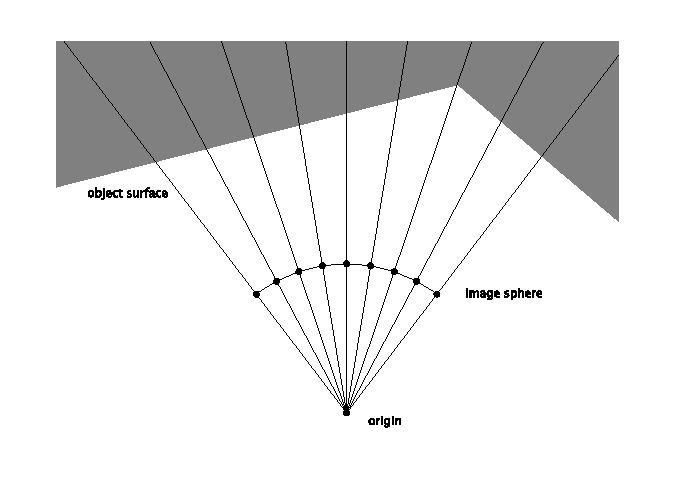
\includegraphics[trim=8mm 1cm 8mm 1cm, crop, width=\linewidth]{fig/cam_range.pdf}
	\caption{Range camera}
\end{subfigure}%
\begin{subfigure}{.33\textwidth}
	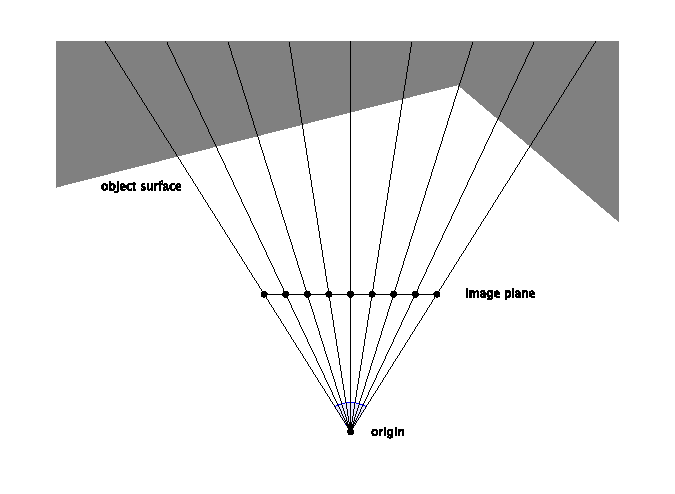
\includegraphics[trim=8mm 1cm 8mm 1cm, crop, width=\linewidth]{fig/cam_perspective.pdf}
	\caption{Perspective camera}
\end{subfigure}%
\begin{subfigure}{.33\textwidth}
	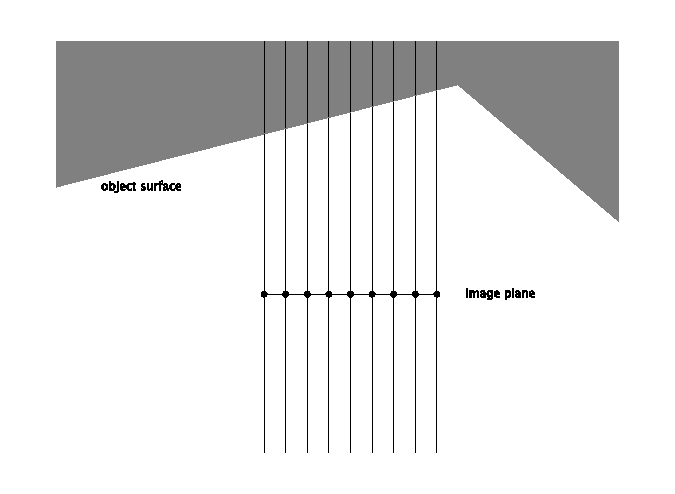
\includegraphics[trim=8mm 1cm 8mm 1cm, crop, width=\linewidth]{fig/cam_parallel.pdf}
	\caption{Parallel camera}
\end{subfigure}
\caption{Illustration of different camera types in 2D}
\end{figure}

The \emph{range camera} does a linear mapping from the angle of the ray to the pixel on the image. The image, when put in three-dimensional space such that the rays pass through its pixels, has the shape of a rectangular sphere section. For the three-dimensional equivalent, additional complexities occur because of the different possible ways to define spherical coordinates. The field of view can cover the entire range of directions. This model corresponds most closely to a real laser scanner.

For the \emph{perspective camera}, the image is a plane instead of a sphere. This corresponds to the way that photographic cameras take pictures. The resulting image contains some distortion relative to the one from the range camera, as the angles between rays get smaller towards the extremities of the field of view. On \emph{parallel camera}, all the rays are parallel. For both the perspective and parallel camera, the mapping from 3D point coordinates to pixel coordinates on the image plane is a linear function and can be described as a multiplication with a $4 \times 4$ matrix in homogeneous coordinates. This is further described in the next sections. For the range camera, trigonometric functions are necessary to describe the mapping.

For the parallel camera, all rays have the direction of the normal vector $\vec{n}$ of the image plane. When considering only a small subregion of the field of view, the rays can also be considered to be parallel by approximation for the range and perspective cameras, as well as for real 3D scanners. Thus for any small part cropped out of a range image point cloud, the camera can be modeled as a parallel camera. These rays will also by approximation be equidistant from each other, and arranged on a square or rectangular grid on an image plane.

This way the point dispersion on small, locally planar surfaces can be modeled using a parallel camera.


\subsection{3D scanner technology}
In general 3D scanners are devices which probe their physical environment in order to collect information about the shape and possibly appearance of objects.

\subsubsection{Laser rangefinder}
A laser rangefinder is a device which uses a laser beam to measure the distance of a physical object. It consists of a laser and an optical sensor pointing in the same direction. A laser beam is sent out to the object, and the \emph{time-of-flight} until the reflected beam is received by the optical sensor is measured. The distance of the object can then be determined by measuring either \emph{time of flight} or the \emph{phase shift}.

For the former case, a short laser pulse is send out, and the time $\Delta t$ until the reflected light hits the sensor is measured. The distance of the object can then be calculated as $d = \frac{c \, \Delta t}{2}$, where $c$ is the speed of light. Using this procedure long distance measurements of up to 10 kilometers can be taken, at a very high rate. However due to the high speed of light, the precision is limited. Obtaining measurements that are accurate within more than a few centimeters requires creating very short laser pulses and precise time measurement.

An alternate method is to use a continuous light beam instead of a short pulse, and measure the phase shift between the emitted and the received signal. This allows for measuring a distance in a range within the wavelength of the emitted light. By sampling the cross-correlation of both signals at different time offsets, a value for the phase shift can be obtained.

\subsubsection{Time-of-flight scanner}
Time-of-flight scanners are based on a laser range finder. A 3D scan is performed by sequentially measuring the distances in different directions in the field of view. The beam is oriented by rotating the rangefinder or using a mirror system. A \emph{range image} is obtained. In spherical coordinates, the radius of each point corresponds to the distance measured by the rangefinder, whereas the azimuth and elevation depends on the direction of the beam. 

These devices are also called \gls{lidar} scanners, especially in applications other than the scanning of solid object surfaces, as mentioned before. This is by analogy to \gls{radar} and \gls{sonar}, which operate in a similar way using radio waves and sound waves to detect objects, respectively.

Time-of-flight scanners are \emph{long-range scanners}. They may operate over distances of several kilometers. However due to the high speed of light, they have a relatively low accuracy on the order of millimeters.

\subsubsection{Triangulation scanner}
Another laser-based technique for recording 3D data is to find the spatial location of the laser dot by triangulation. As with the time-of-flight scanner, a laser beam is sequentially projected in different directions onto the object. But instead of measuring the return time of the beam, a camera is used to track the location of the laser dot on the object surface. The projected two-dimensional position of the laser dot is thus known from both the point of view of the laser and the point of view of the camera. Also the pose of the camera relative to the laser is fixed. These three pieces of information are sufficient to calculate the three-dimensional location of the laser dot on the object surface.


\section{Operations on point clouds}
This section describes some of the operations that are applied to point cloud data during the post-processing of 3D scans. The point cloud is regarded as an unordered set $P = \{ (x_i, y_i, z_i) \}$. In the chapter \ref{ch:implementation} data structures used to lay the point set out in memory are considered.


\subsection{Basic operations}

\subsubsection{Fusion}
Since point clouds are unordered point sets, fusing two point clouds corresponds to taking the union of the two sets.

When two point clouds represent different views of the same object and the goal is to get a point cloud the covers a greater part of the object, they must first be \emph{registered} and put into the same coordinate system.

Fusing creates some redundancy in the overlapping parts of the point clouds. Techniques exist to refine the resulting distribution and density of points, as described for example in \cite{Fuhr2011} and \cite{Kyos2013}.


\subsubsection{Transformation}
To apply an affine transformation to the object represented by the point cloud, the same transformation matrix is simply applied to each point. The transformation will be relative to the origin point of the point cloud. When the points are attributed with normal vectors, the linear part of the transformation (i.e. not the translation) also needs to be applied to them.

For point cloud registration, a rigid transformation will be applied to one \emph{loose} point cloud to put it into the coordinate system of the \emph{fixed} point cloud.


\subsubsection{Cropping}
Cropping means to simply remove the points from $P$ that lie outside some geometric region. This region may be a bounding box, a view frustum of a camera or other. It is typically performed manually using point cloud software as a first step in post-processing the 3D scans.

When done on a range image, the coordinate system must be maintained since the camera will still be at the origin, which can be far off the cropped area.


\subsubsection{Closest point finding}
Finding for any \emph{position} $(x, y, z)$, the point $p \in P$ closest to it. This can implemented efficiently by using a tree structure representation of the point cloud, as will be described in a later chapter.

Usually the Euclidian distance between points is used, though for some applications other distance metrics are useful as well.


\subsubsection{Nearest neighbor finding}
Finding for any \emph{point} $p' \in P$ in the point cloud, the point $p \in P$ other than itself that is closest. For many applications it is useful to find the $k$ nearest neighbors, either for one point, or for a whole set of points.

Also here, different data structures allow for implementing this in an efficient manner. Different optimizations are possible here than for the closest point problem, because $p'$ must be a point of the point cloud, and not just any position in space.


\subsection{Computation of normal vector}
Computing a estimation of the normal vector of the surface at a given point $p \in P$. Different approaches exist, and because the surface is unknown there is not necessarily a best method or a clear way to evaluate its accuracy.

One basic approach is to compute the $k$ nearest neighbors for some value $k$, and then take the normal vector of a plane fitted to those $k + 1$ points. This plane fitting can be done using a \gls{ransac} or a least squares-based approach. The calculation must be insensitive to outliers, in particular cases where two surfaces intersect and near sharp edges of surfaces.

For range image, the normal vector of a point can also be used on the two-dimensional image space. The rectangular neighborhood of a pixel corresponds to an approximation of the nearest neighbors of the point. Using the gradient or other measures on the pixels' depth values, an estimation of the normal vector can be made.

Other per-point values such as a local density or curvature measure can be useful, and a version for those two will be defined chapter \ref{ch:analysis_pc}.


\subsection{Projection}
Generating a virtual \emph{range image} from the point cloud. As described above, a range image contains only the part of the object that is visible from a given viewpoint. Each point in the range image corresponds to a two-dimensional coordinate on a pixel grid. In range images produced by real 3D scanners, the precise mapping from pixel coordinates to the azimuth and elevation components of the point's spherical coordinates may be unknown.

Here, projection essentially means to simulate the operation on a 3D scanner, with the point cloud replacing the real object. The range image obtained from projecting a point cloud using should ideally be the same as would be obtained from scanning the real object with a scanner having the same pose and coordinate mapping parameters. However the point cloud contains only a sparse set of point representing the surfaces, without direct connectivity information.

Let $w, h \in \mathbb{N}$ be the width and height of the image. The aim of a projection algorithm is to implement a function $r : [0, w[_{\mathbb{N}} \times [0, h[_{\mathbb{N}} \rightarrow P \cup \{ \epsilon \}$, which associates to each image pixel a point from the point cloud $P$, or the invalid point $\epsilon$. 

Let $\mathbf{proj}_{C} : \mathbb{R}^3 \rightarrow \mathbb{N}^2 \cup \{ \epsilon \}$ be the function used to map 3D coordinates to pixel coordinates. $C$ represents the pose and parameters of the virtual camera. So $(0, 0) \leq \mathbf{proj}(\cdot) < (w, h)$. For each image coordinate $(x_i, y_i)$, the region of space where points would map onto that pixel is given by $\{ p \in \mathbb{R}^3 : \mathbf{proj}_{C}(p) = (x_i, y_i) \}$. In the case of perspective projection, it will have the shape of a thin square-base frustum extending from the camera point to infinity. In orthogonal projection, it instead corresponds to a thin cuboid. The discrete subset of points from the point cloud $P$ which lie in that region is given by $P_{(x_i,y_i)} = \{ p \in P : \mathbf{proj}_{C}(p) = (x_i, y_i) \}$.

Figure \ref{fig:pp_projection} shows the situation in 2D for a perspective position. Two surface parts of the object lie inside the frustum. The further one is called $A$ and the closer one $B$.

\begin{figure}[h]
\center
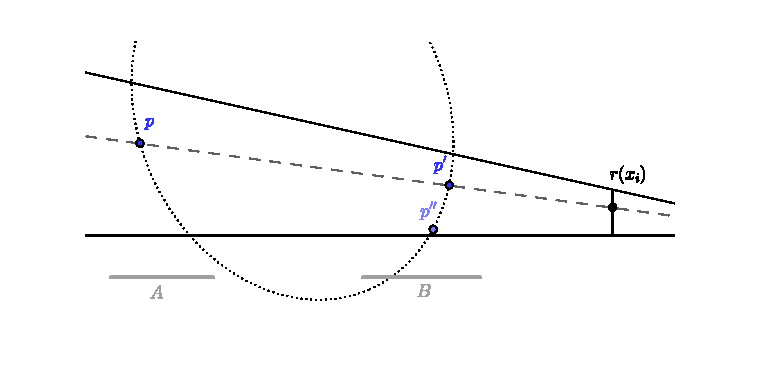
\includegraphics[width=.8\textwidth]{fig/pp_projection.pdf}
\caption{Illustration of point cloud to range image projection in 2D}
\label{fig:pp_projection}
\end{figure}

A simple approach to define the function $r$ is to let $r(x_i, y_i)$ be the point in $P_{(x_i,y_i)}$ that is closest to the camera, or $\epsilon$ when $P_{(x_i,y_i)}$ is empty. If $P_{(x_i,y_i)}$ was not a discrete set, but instead an uncountable set of surface points, it would be guaranteed that the chosen point $p$ if not occluded by another point $p'$ lying in front of it, because $p'$ would necessarily also be in $P_{(x_i,y_i)}$.

Choosing the closest point is not necessarily the best approach. Another point $p''$ might be a better candidate, when evaluating additional attributes of the points. Also the closest point may be an outlier located in front of $B$. Another approach can be to group several points and generate a new one. The important thing is that the point lies on surface $B$.

But because $P_{(x_i,y_i)}$ are discrete sets, if the point density is not high enough, it can occur that no point in it lies on surface $B$, and so instead one in $A$ would be chosen.



\subsection{Registration} \label{sec:pc_registration}
Given two point clouds $P$ and $Q$ that represent the same object, find a translation and rotation that will put both point clouds into the same coordinate system, and thus align the corresponding parts. $P$ and $Q$ are be taken from different poses, so different parts of the object are occluded in the two point clouds.

For example to obtain a full point cloud of a solid object, it needs to be scanned from different sides. Before it can be merged into a full point cloud, the precise relative poses of the scans need to be known. The aim of a registration algorithm is to compute an estimation of those poses.

Many different methods exist. A large survey of registration methods is given in the next chapter \ref{ch:pcreg}.



\subsection{Other operations}

\subsubsection{Image-to-cloud registration}
Wrapping a photographic image on a point cloud, for example with the goal of attributing colors to points from a raw scan. This involves photogrammetric and image analysis techniques for finding correspondences between the point cloud and the image.


\subsubsection{Meshing}
Adding connectivity to the points, by constructing a triangular mesh that joins together neighboring points on the same surfaces. 


\subsubsection{Outlier removal}
Identifying the filtering out outliers from the point cloud. A basic technique would be to remove every point whose distance to its closest neighbor is above a given threshold. This threshold distance could be fixed in function of the average, or median nearest neighbor distances of all the points.

This technique would not be able to filter out clusters of outliers that lie close to each other. Many better methods have been developed, for example \cite{Soto2006}.

Outlier removal can be a necessary step before applying a registration algorithm.

\subsubsection{Down-sampling}
Reducing the density of the point cloud. The most simple method is \emph{random down-sampling}, in which every point is removed at a fixed probability $p < 1$. It is also possible to select random points to remove such that a deterministic number of points is removed in the end. Random down-sampling leads to an irregular point dispersion pattern, with non-uniform density.

Another possibility is to put a regular lattice of small, equal-volume cubic cells into the coordinate system, and keep only one point per cell.

When working with range images, down-sampling is best done on the image space, by reducing the image size using nearest neighbor interpolation. Bilinear or bicubic interpolation would introduce new depth values and thus add false points into the point cloud.

\subsubsection{Super-resolution}
Increasing the density of the point cloud, by introducing new, artificial points between gaps. Methods have been developed to use auxiliary data, for example photographs of the same object, to increase the resolution of range images. For example \cite{Yang2007}, \cite{Bart2009}, \cite{Soh2012} and \cite{Lo2013}.

Approaches that do not use auxiliary data, but do an estimative super-resolution of the range image are also possible, like for example \cite{Do2012}

\section{Transformation matrices and homogeneous coordinates}
Positions in three-dimensional space can be represented using cartesian coordinates. Let $O$ be an origin point in space, and let $\vec{i}, \vec{j}, \vec{k}$ be three orthogonal vectors of norm $1$. Then $\vec{p} = (x, y, z)$ represents the position $O + x \, \vec{i} + y \, \vec{j} + z \, \vec{k}$. The vectors $\vec{o}, \vec{i}, \vec{j}, \vec{k}$ define the coordinate system.

A point cloud as defined as a set of points, where each one has a position and possibly additional attributes. The positions in one point cloud are all set in the same coordinate system. When the points are attributed with normal vectors, or other vector-type attributes, this is also true for them. Applying a transformation $\matr{T}$ to a point cloud means applying that transformation to the position, and to any vector-type attributes of it.

\subsection{Classification}
The transformations used here are classified as follows:

\begin{figure}[h]
\center
\includegraphics[width=.8\textwidth]{fig/transformations_venn.pdf}
\caption{Venn diagram of three-dimensional transformations}
\end{figure}

\emph{Linear} transformations correspond to a linear recombination of the three coordinates, and can be expressed using a $3 \times 3$ transformation matrix. \emph{Affine} transformations are linear transformation with an additional translation. A \emph{rigid} transformation is an affine transformation where the linear part is an orthogonal matrix. It preserves the distance between every pair of points. \emph{Proper rigid} transformations exclude reflection, and consist of a rotation and a translation. They correspond to the movement an object can make in three-dimensional space without altering its shape. A \emph{projective} transformation is an affine transformation, followed by a division of the three coordinates by one same linear combination of the coordinates. It can for instance express perspective projections. Additionally, the term \emph{non-rigid} transformation is sometimes used in the context of point cloud registration, to express any transformation (not necessarily affine) that alters the shape of the model.

Transformations can be combined into a conjunction of transformations, which would be classified into the lowest common class of its components. For instance a translation followed by a reflection would be a rigid transformation that is neither linear nor proper rigid. Conjunctions of transformations are in general not commutative, but for all possible orders of application the results belong to the same class.

\subsubsection{Linear transformation}
A linear transformation is one where each coordinate of a point is mapped to a linear combination of the three coordinates. As such it can be expressed using a $3 \times 3$ matrix, and applying the transformation corresponds to multiplying this matrix $\mat{T}$ by column vector formed by the point coordinates.
\begin{equation}
\left[ \begin{matrix}
	t_{1,1} & t_{1,2} & t_{1,3} \\
	t_{2,1} & t_{2,2} & t_{2,3} \\
	t_{3,1} & t_{3,2} & t_{3,3}
\end{matrix} \right] \times
\left[ \begin{matrix} x \\ y \\ z \end{matrix} \right] = 
\left[ \begin{matrix}
	t_{1,1} \, x + t_{1,2} \, y + t_{1,3} \, z \\
	t_{2,1} \, x + t_{2,2} \, y + t_{2,3} \, z \\
	t_{3,1} \, x + t_{3,2} \, y + t_{3,3} \, z
\end{matrix} \right]
\end{equation}
So in a transformation $\vec{p'} = \matr{T} \, \vec{p}$, $t_{i,j}$ indicates the coefficient of the $j$-th coordinate of $\vec{p}$ in the $i$-th coordinate of $\vec{p'}$. As a consequence the origin $(0, 0, 0)$ is a fixed point in any linear transformation. Linear transformations can for example express a rotation, a shearing, a reflection, or an orthogonal projection. Because of the associativity of matrix multiplication, the composition of linear transformations can be expressed in one single linear transformation matrix. First applying $\matr{T_1}$ followed by $\matr{T_2}$ is the same as applying $\matr{T_2} \times \matr{T_1}$, because
\begin{equation}
	\vec{p'} = \matr{T_2} \, ( \matr{T_1} \, \vec{p} ) = (\matr{T_2} \, \matr{T_1}) \, \vec{p}
\end{equation}

Also, the inverse transformation is expressed by the inverse of the transformation matrix $\matr{T^{-1}}$. As mentioned, the conjunction of two linear transformations is non-commutative, just like the underlying matrix multiplication.

\subsection{Rotation}
In two-dimensional euclidian geometry, a rotation around the origin point $(0, 0)$ with angle $\theta$ is expressed by the linear transformation matrix
\begin{equation}
\matr{R}_{\theta} = \left[ \begin{matrix}
	\cos \theta & - \sin \theta \\
	\sin \theta & \cos \theta
\end{matrix} \right]
\label{eq:rotation-matrix-2d}
\end{equation}
This can be derived using the geometric definition of the trigonometric functions. In three-dimensional additionally a plane of rotation, of equivalently an axis of rotation needs to be specified. The linear transformation matrices for the \emph{elemental rotations} around the \emph{x}, \emph{y} or \emph{z} axis can be deduced from \ref{eq:rotation-matrix-2d} by keeping one coordinate unchanged and applying the 2D rotation on the plane formed by the other two:
\begin{equation}
\matr{R}_{\theta}^x = \left[ \begin{matrix}
	1 & 0 & 0 \\
	0 & \cos \theta & - \sin \theta \\
	0 & \sin \theta & \cos \theta
\end{matrix} \right]
\hspace{1cm}
\matr{R}_{\theta}^y = \left[ \begin{matrix}
	\cos \theta & 0 & \sin \theta \\
	0 & 1 & 0 \\
	- \sin \theta & 0 & \cos \theta
\end{matrix} \right]
\hspace{1cm}
\matr{R}_{\theta}^z = \left[ \begin{matrix}
	\cos \theta & - \sin \theta & 0 \\
	\sin \theta & \cos \theta & 0 \\
	0 & 0 & 1
\end{matrix} \right]
\end{equation}

\subsubsection{Euler angles}
One common way to express a three-dimensional rotation is using \emph{Euler angles}, that is, the angles by which to rotate around those three axis. For example, $(\phi, \theta, \psi)$ may express the rotation $\matr{R}_{\phi}^x \, \matr{R}_{\theta}^y \, \matr{R}_{\psi}^z$. Because of the non-commutativity, many different conventions are possible: The three elementary rotations can be applied in different orders, such as \emph{x-y-z}, \emph{z-y-x} or \emph{x-y-z}. Also combinations of only two elementary rotations like \emph{x-y-x} or \emph{z-x-z} are possible, where the same axis used for the first and third rotation. In expression like $\matr{R}_{\phi}^x \, \matr{R}_{\theta}^y \, \matr{R}_{\psi}^z$, the three elementary rotations are \emph{intrinsic}: The second rotation rotates around the new \emph{y} axis, which has already been displaced from the first rotation. In an \emph{explicit} conventions, all three rotations instead take place in a fixed coordinate system.

The terms \emph{yaw}, \emph{pitch} and \emph{roll} are commonly used to name the three rotation angles. Given an object pointing into a certain direction in space, such as a camera or a moving vehicle, \emph{roll} refers to a rotation around the axis in which it is pointing. \emph{Pitch} is a rotation around its relative horizontal axis, and \emph{yaw} around its relative vertice axis. For example, a \emph{pitch} rotation of an aircraft would make it fly upwards or downwards.

Besides the many possible conventions, another problem with Euler angles is the \emph{gimbal lock} phenomenon, where two components can end up representing a rotation around the same axis. Because of gimbal lock, and because the angles are taken modulo $2\pi$, small changes in a rotation do not always correspond to small changes in the Euler angles. This makes them unsuited for processing rotations algorithmically and for solving optimisation problems. Instead, a good alternative to directly working with rotation matrices is to use quaternions, which express the rotation using $4$ real values.

\subsubsection{Rotation around an axis}
A rotation can also be represented as axis of rotation $\vec{\omega}$, and an angle $\theta$ around that axis. Using \emph{Rodrigues' rotation formula} the image $\vec{p'}$ of point $\vec{p}$ can be calculated as
\begin{equation}
\vec{p'} = (\cos \theta) \vec{p} + (\sin \theta) (\vec{\omega} \times \vec{p}) + (1 - \cos \theta) (\vec{\omega} \vec{p}) \vec{\omega}
\end{equation}

This translates directly to the rotation on a plane, by setting $\vec{u}$ to be the normal vector of that plane.


\subsubsection{Rotation between two vectors}
There are infinitely many possible rotations that map a vector $\vec{v}$ into another vector $\vec{u}$. $\vec{v}, \vec{u}$ are two linearly independent unit vectors. One preferred rotation can be chosen which fixes the plane spanned by $\vec{v}$ and $\vec{u}$.

Its axis of rotation is calculated using the cross product $\vec{\omega} = \vec{v} \times \vec{u}$, and the angle using the dot product $\theta = \arccos (\vec{v} \vec{u})$.


\subsubsection{Quaternions}
The quaternions $\mathbb{H}$ are a four-dimensional extension of the complex numbers, using four imaginary units $i, j, k$. The multiplication rules of the imaginary units, and the real unit $1$ are defined by the fundamental formula
\begin{equation}
i^2 + j^2 + k^2 + i j k = -1
\end{equation}
Unlike with the real or complex numbers, quaternion multiplication is not commutative.

Unit quaternions are quaternions of norm one. They can be used to represent three-dimensional rotations and map directly to the angle-axis representation, using
\begin{equation}
\dot{q} = \left( \cos \tfrac{\theta}{2}, \omega_x \sin \tfrac{\theta}{2}, \omega_y \sin \tfrac{\theta}{2}, \omega_z \sin \tfrac{\theta}{2} \right)
\end{equation}

A composition of rotations corresponds to the product of the quaternions, and the inverse of a quaternion corresponds to the inverse rotation. Representing rotations using quaternions is a good compromise between Euler angles and rotation matrices: There is no gimbal lock, and the representation is more compact as rotation matrices. It can also be more numerically stable as less operations are involved in computing the composition or inverse of a rotation. Applying the rotation to a point using its quaternion representation amounts to two quaternion multiplications, or alternately the quaternion can be converted to a rotation matrix.


\subsection{Interpolation of rotation} \label{sec:rot_interp}
Interpolating a translation can be done simply by linear interpolation of its three components: $\vec{t}(t) = (1 - t) \, \vec{t}_\text{min} + t \, \vec{t}_{\text{max}}$. By the distributivity of matrix by vector multiplication, this is invariant of the coordinate system. But interpolating a rotation or a complete rigid transformation is more complicated. A linear interpolation of the Euler angles, the quaternion components, or the transformation matrix components generally does not product a smooth animation because of the gimbal lock phenomenon, or because the transformation does not remain rigid.

Informally, an interpolation should such that an object whose pose changes in time between the two ends of the interpolation, moves smoothly at about a constant speed, the same way as one would manually place a real object from one pose into another.

Quaternions allow for defining a smooth interpolation between two rotations, called the \emph{spherical linear interpolation}, or \emph{slerp}. It is such that movements along unit-radius great circle arcs retain a constant speed. Using quaternions, it is defined as
\begin{equation}
s(\dot{q}_0, \dot{q}_1, t) = \dot{q}_0 (\dot{q}^{-1}_0 \dot{q}_1)^t
\end{equation}
for $0 < t < 1$.

Quaternion exponentiation is defined using $\dot{q}_t = e^{\dot{q} \, \log t}$, where the quaternion exponential function can be written using the power series
\begin{equation}
e^{\dot{q}} = \sum_{n=0}^{\infty} \frac{\dot{q}^n}{n!}
\end{equation}


\subsection{Affine transformation}
Translations are not linear transformations, because they add a constant term to each coordinate of $\vec{p'}$. An \emph{affine} transformation corresponds to a linear transformation followed by a translation: $\vec{p'} = \matr{T} \, \vec{p} + \vec{t}$. Let $\vec{p'} = \matr{T_1} \, \vec{p} + \vec{t_1}$ and $\vec{p''} = \matr{T_2} \, \vec{p'} + \vec{t_2}$ be the expressions of two subsequent affine transformation to apply to $\vec{p}$.
\begin{equation}
	\vec{p''} = \matr{T_2} \, (\matr{T_1} \, \vec{p} + \vec{t_1}) + \vec{t_2} = (\matr{T_2} \, \matr{T_1}) \, \vec{p} + (\matr{T_1} \vec{t_1} + \vec{t_2})
\end{equation}
So a composition of multiple affine transformations is still an affine transformation, but the translation vectors cannot be simply added up. It can be seen that the composition is again non-commutative, except for the case when $\matr{T_2} = \matr{T_1} = \matr{I}$, that is, when both transformations are translations only.

Also if the translation component is applied \emph{before} the linear component (instead of \emph{after} it), it represents a different affine transformation:
\begin{equation}
	\matr{T} \, (\vec{p} + \vec{t}) = \matr{T} \, \vec{p} + \matr{T} \, \vec{t} \neq \matr{T} \, \vec{p} + \vec{t}
\end{equation}


\subsubsection{Rigid transformation}
The subclass of affine transformation where $\matr{T}$ is an orthogonal matrix are the rigid transformations. By definition, its row vectors, and its column vectors are orthogonal unit vectors. Orthogonal matrices preserve the dot product of vectors, and as a consequence distances and angles between any two pairs of points are preserved. Orthogonal matrices represent either a rotation or a reflection, and its determinant $\det(\matr{T})$ is always either $+1$ for a rotation or $-1$ for a reflection. This is a necessary but not sufficient condition, as there are also non-orthogonal matrices with determinant $+1$ or $-1$. So a rigid transformation can be a translation, rotation, reflection, or any composition thereof.

A proper rigid transformation is defined as a rigid transformation for which $\matr{T}$ is a rotation matrix. It always consists of a rotation and a translation, and any composition of proper rigid matrices can be reformulated as a single rotation and translation:
\begin{equation}
	\matr{R_2} \, (\matr{R_1} \, \vec{p} + \vec{t_1}) + \vec{t_2} = (\matr{R_2} \, \matr{R_1}) \, \vec{p} + (\matr{R_2} \, \vec{t_1} + \vec{t_2})
\end{equation}
Where $\matr{R_2} \, \matr{R_1}$ is also an orthogonal matrix, it being the composition of two rotations.

Proper rigid transformations correspond to the ways a real object can be moved in three-dimensional space without altering its shape. As such, they can be used to represent the position and orientation of an object.

In the following text, the term ``rigid transformation'' will always refer to a proper rigid transformation.

In most use cases involving three-dimensional geometry, non-proper rigid transformations are rarely used since they change the handedness of an object, which is in reality not possible in three-dimensional space. In fact, with a fourth spatial dimension it would be possible with a 4D rotation that temporarily pulls the object out of the three-dimensional subspace. This process would not alter the object's internal structure. But while both the start and end state would be possible in 3D space, the intermediary steps are not, and movements in reality are always continuous.

\subsection{Homogeneous coordinates}
In order to simplify calculations and notation, it is natural to use \emph{homogeneous coordinates}. They allow for affine and projective transformations to be written using a single $4 \times 4$ matrix.

Formally, a vector $\homvec{v}$ in homogeneous coordinates corresponds to a vector $\vec{v}$ in cartesian coordinates iff
\begin{equation}
	\homvec{v} = \colvecT{x, y, z, w}
	\hspace{1cm}\mathrm{and}\hspace{1cm}
	\vec{c} = \colvecT{\frac{x}{w}, \frac{y}{w}, \frac{z}{w}}
\end{equation}

The conversion from homogeneous to cartesian coordinates consists of an element-wise division by the fourth component $w$ of the vector itself. This non-linear operation cannot be represented by cartesian matrix multiplications alone. The equivalent in homogeneous coordinates of an affine transformation given by the linear transformation $\matr{L}$\footnote{Using $\matr{L}$ here instead of $\matr{T}$.}, and the translation vector $\vec{t}$, where the linear transformation is applied before the translation, is the $4 \times 4$ matrix
\begin{equation}
	\hommatr{T} = \left[ \begin{matrix}
		l_{1,1} & l_{1,2} & l_{1,3} & t_1 \\
		l_{2,1} & l_{2,2} & l_{2,3} & t_2 \\
		l_{3,1} & l_{3,2} & l_{3,3} & t_3 \\
		0 & 0 & 0 & 1
	\end{matrix} \right]
\end{equation}
A distinction is made between positions and vectors: When transforming a position, with the linear transformation is applied, followed by the translation. For vectors on the other hand, only the linear transformation is applied. A vector does not represent a position in space, but only a direction and norm. Its coordinates represent the position of its end point, assuming that its start point is at $\colvecT{0, 0, 0}$. For example when applying a rigid transformation to a point cloud where points are attributed with surface normal vectors, the point positions should get rotated and then translated. The normal vectors should be rotated the same way, but no translation vector should be added to them.

Positions are converted into homogeneous coordinates by adding an extra component $w = 1$, whereas for vectors an extra component $w = 0$ is added. The three first components $x, y, z$ remain the same. It can be seen that
\begin{equation}
\left[ \begin{matrix}
	x \\ y \\ z \\ 1
\end{matrix} \right] \times  \left[ \begin{matrix}
	l_{1,1} & l_{1,2} & l_{1,3} & t_1 \\
	l_{2,1} & l_{2,2} & l_{2,3} & t_2 \\
	l_{3,1} & l_{3,2} & l_{3,3} & t_3 \\
	0 & 0 & 0 & 1
\end{matrix} \right] = \left[ \begin{matrix}
	l_{1,1} \, x + l_{1,2} \, y + l_{1,3} \, z + t_1 \\
	l_{2,1} \, x + l_{2,2} \, y + l_{2,3} \, z + t_2 \\
	l_{3,1} \, x + l_{3,2} \, y + l_{3,3} \, z + t_3 \\
	1
\end{matrix} \right] \coreq \left[ \begin{matrix}
	l_{1,1} \, x + l_{1,2} \, y + l_{1,3} \, z + t_1 \\
	l_{2,1} \, x + l_{2,2} \, y + l_{2,3} \, z + t_2 \\
	l_{3,1} \, x + l_{3,2} \, y + l_{3,3} \, z + t_3 \\
\end{matrix} \right]
\end{equation}
In the case where $w = 0$, the components of $\vec{t}$ get removed. In the case of affine transformations, the last row of the homogeneous matrix is always $\rowvec{0, 0, 0, 1}$, and no division takes place. For perspective projections, a division by the $z$ component will compute foreshortening.

Because here an affine or projective transformation is applied by single matrix multiplication, is follows that any composition of those matrices can be represented using the matrix product of multiple $4 \times 4$ matrices.

\subsection{Pose}
This position and orientation of an object in space is called its \emph{pose}. A pose is also a cartesian coordinate system. Coordinates as well as other poses are always defined relative to such a coordinate system.

In any sufficiently complex three-dimensional environment, it becomes natural to define the positions and orientations of object relative to each other, and not in a single global coordinate system. 3D modelling software such as \emph{Blender} typically implement a tree-structure of objects, in which the pose of each object is defined relative to its parent. A similar software system was written for this project, as will be described in chapter \ref{ch:implementation}.

The problem of 3D scan registration treated in this paper is precisely to find the pose from which a scan was taken, relative to another scan, and the output of any point cloud registration algorithm is a rigid transformation matrix.

A pose corresponds to an orthonormal coordinate system which is defined by tuple $S = \langle O, \vec{i}, \vec{j}, \vec{k} \rangle$ where $O$ is the origin point, and $\vec{i}, \vec{j}, \vec{k}$ three orthogonal vectors with $\|\vec{i}\| = \|\vec{j}\| = \|\vec{k}\| = 1$. The origin point and the vectors of a coordinate system are defined within its \emph{parent} coordinate system. The root coordinate system in that tree is called \emph{world space}. For an \emph{identity} coordinate system, $O = (0, 0, 0)$, $\vec{i} = \colvecT{1, 0, 0}$, $\vec{j} = \colvecT{0, 1, 0}$ and $\vec{k} = \colvecT{0, 0, 1}$.

A pose can also be expressed using the \emph{transform-to-parent} rigid transformation $\matr{M}$, which transforms the coordinates of points or vectors expressed in its coordinate system $S_i$, into the coordinates of the same point of vector in its parent coordinate system $S_{i-1}$. Equivalently, the \emph{transform-from-parent} rigid transformation is its inverse $\matr{M^{-1}}$. Then
\begin{equation}
	O_{i} = \matr{M^{-1}} \, O_{i-1}
	\hspace{1cm}
	\vec{i_{i}} = \matr{M^{-1}} \, \vec{i_{i-1}}
	\hspace{1cm}
	\vec{j_{i}} = \matr{M^{-1}} \, \vec{j_{i-1}}
	\hspace{1cm}
	\vec{k_{i}} = \matr{M^{-1}} \, \vec{k_{i-1}}
\end{equation}
where the distinction between positions and vectors using homogeneous coordinates is made.

Transformation matrices that express position in one coordinate system in another coordinate system are computed by traversing the tree, and calculating a conjunction of transform-to-parent and transform-from-parent matrices.


\section{Least squares method}
The least squares method is a way to calculate an approximate solution to an overdetermined system. For example the equation $y = ax + b$ of a line that crosses two points $(x_1, y_1)$ and $(x_2, y_2)$ can easily be calculated by solving a linear system with 2 equations and 2 unknowns. But if there are 3 or more points, there is no solution unless the points are perfectly aligned. Here a least squares solution would be the line which minimizes the sum of the squares of the distances of the points to itself.

Formally, let $\{ (x_i, y_i) \}$ be a set of $n$ data points. $x_i$ are independent variables and $y_i$ dependent variables found by observation. Both $x_i$ and $y_i$ can be vectors. For example the problem of fitting a plane to a set of 3D points may be modelled with $x_i$ being a data point's X coordinate, and $\vec{y_i}$ that data point's Y and Z coordinates.

The goal is to find a vector of parameters $\beta$ that define a model $\hat{y}_i = f_{\beta}(x_i)$. Because in general there is no $f_{\beta}$ for which $\forall i, \hat{y}_i = y_i$, one searches a solution that minimizes the sum of the squared residuals:
\begin{equation}
\hat{\beta} = \argmin_{\beta} S \hspace{7mm} \text{where} \hspace{7mm} S = \sum_{i=1}^{n} (y_i - \hat{y}_i)^2
\end{equation}
For the example where the model is a line, one can define $\beta = (a, b)$ and $f_{\beta}(x) = ax + b$. Then the residual would be the vertical distance of a point to a line. It is also possible to define a linear expression of $f_{\beta}$ by which the orthogonal distances of the points to the lines are minimised. Many similar geometrical fitting problems can be solved in this manner, such as fitting a plane, circle, sphere, or other object to a set of points. \cite{Eber1999}

\subsection{Linear least-squares}
In general, a solution for least square problems can be computed by setting the gradient $\nabla S$ to zero. Since the terms $y_i$ are constant, this becomes for each component $\beta_j$:
\begin{equation} \label{eq:lsq_sol}
\frac{\partial S }{\partial \beta_j} = -2 \sum_{i=1}^{n} \frac{\partial f_{\beta}(x)}{\partial \beta_j} = 0
\end{equation}

If $f_{\vec{\beta}}$ is a linear combination of the parameters $\vec{\beta}$, then a closed form expression for the solution exists. Let there be $n$ data points $(x, y)$, where $x$ are vectors of $m$ components, and $y$ real numbers. (Here the subscript refers to the component of the vector $x$, not the index of the data point). $\beta$ will also have $m$ components. The function $f_{\beta}$ is of the form
\begin{equation} \label{eq:lsq_linf}
f_{\beta}(x) = \beta_1 \, x_1 + \beta_2 \, x_2 + \dots + \beta_m \, x_m
\end{equation}
For the example of fitting a line to a set of 2D points, one would add a second component to the dependent variables which is always set to $1$, so as to get back to $f_{\beta}(x) = ax + b$.

The overdetermined system to solve can be written in matrix form
\begin{equation}
\matr{X} \, \hat{\beta} = \vec{y}
\end{equation}
where $\matr{X}$ is a $n \times m$ matrix. Each row corresponds to a data point, and each component per row corresponds to the $j$-th component $x_j$ of the dependent variable of that data point. The sum of squares $S$ to minimize becomes
\begin{equation}
S = \sum_{i=1}^{n} \| y_i - \sum_{j=1}^{m} X_{i,j} \beta_{j} \|^2 = \| y - \matr{X} \, \vec{\beta} \|^2
\end{equation}
From \ref{eq:lsq_linf}, the partial derivative of a residual becomes
\begin{equation} \label{eq:lsq_linr}
\frac{\partial (y_i - f_{\beta}(x))}{\partial \beta_j} = - X_{i,j}
\end{equation}
Putting \ref{eq:lsq_linr} into \ref{eq:lsq_sol} and rearranging the expression, one obtains the \emph{normal equations}:
\begin{equation}
\sum_{i=1}^{n} \sum_{k=1}^{m} X_{ij} \, X_{ik} \, \hat{\beta}_k = \sum_{i=1}^{n} X_{ij} \, y_{i}
\hspace{7mm} \text{for} \hspace{7mm}
j = 1, 2, \dots, m
\end{equation}
Written in matrix form:
\begin{equation}
(\transpose{\matr{X}} \, \matr{X}) \, \hat{\beta} = \transpose{\matr{X}} \, \vec{y}
\end{equation}
And so the parameters $\hat{\beta}$ for which $f_{\hat{\beta}}(x)$ is a least squares solution to a linear system can be computed using the closed form expression
\begin{equation}
\hat{\beta} = (\transpose{\matr{X}} \, \matr{X})^{-1} \, \transpose{\matr{X}} \, \vec{y}
\end{equation}

\subsection{Non-linear least squares}
When $f_{\beta}$ is not a linear combination of $x_1, x_2, \dots, x_m$ a closed form solution is generally not possible. Instead it can be computed using the \emph{Gauss-Newton algorithm}, by iterative numerical approximation.

\subsection{Weights}
The least squares methods finds a solution for which the squared residual $(y_i - \hat{y}_i)^2$ is minimized and evenly distributed among all data points. Weights can be added to introduce bias towards higher weight data points, letting their residual become smaller and the others' larger.

For each data point a \emph{weight} $w_i \in \mathbb{R}$ is defined. When $w_i = k \times w_j$ for $k \in \mathds{N}$, the effect is the same as adding $k$ times the data point $(x_i, y_i)$. With weights, the sum to minimize is
\begin{equation}
S = \sum_{i=1}^{n} w_i \, (y_i - \hat{y}_i)^2
\end{equation}
By distributivity, when all $w_i$ become $\lambda w_i$, $S$ becomes $\lambda S$, which doesn't change the minimization problem. Supposing that $w_i$ are rational numbers (which can approximate real numbers to an arbitrary precision), then there exists $\lambda$ such that $\lambda w_i \in \mathbb{N}$. This justifies the previous statement about data points duplication. 

\section{Point set alignment using singular value decomposition} \label{sec:lsq_align}
For point cloud registration, corresponding points $(\vec{p_i}, \vec{q_i})$ of two point clouds are used to find a rigid transformation $\matr{M}$ that aligns the two point clouds. When there are exactly three pairs of points, an exact solution can be found using vector algebra. \cite{Horn1986} For more than three points, a least squares solution can be found.

Here $f_{\beta}(\vec{q}) = \matr{M} \, \vec{q} = \matr{R} \, \vec{q} + \vec{t}$ is the function that applies the sought after rigid transformation. The parameter vector $\beta$ has 6 components, three for the translation and three for the rotation. $\matr{R}$ is the rotation matrix and $\vec{t}$ the translation vector. The independent variable is $\vec{q_i}$, a 3-vector with the coordinates of a point. The dependent variable is $\vec{p_i}$, also a 3-vector with the coordinates of the corresponding point from the other point cloud.

Because the independent variables are vectors, the residuals to minimize are the squares of the norms of the vector differences. The sum $S$ to minimize becomes
\begin{equation}
S = \sum_{i=1}^{n} w_i \, \| \vec{p_i} - (\matr{R} \, \vec{q_i} + \vec{t}) \|^2
\end{equation}

One common approach to calculate the least squares solutions $\matr{R}$ and $\vec{t}$ is to use the following steps:
\begin{enumerate}
\item First the centroids of both point sets are calculated $\vec{c_p} = \frac{1}{N} \, \sum_{i=1}^{n} \vec{p_i}$ and $\vec{c_q} = \frac{1}{N} \, \sum_{i=1}^{n} \vec{q_i}$
\item The points in $P$ and $Q$ are now translated to put the centroid at origin. The translated points are $\vec{p'_i} = \vec{p_i} - \vec{c_p}$ and $\vec{q'_i} = \vec{q_i} - \vec{c_q}$
\item Now the $3 \times 3$ \emph{covariance matrix} is calculated, using $\matr{K} = \sum_{i=1}^{n} w_i \, \vec{p'_i} \, \transpose{\vec{q'_i}}$
\item Different approaches exist to extract the optimal rotation matrix $\matr{R}$ from $\matr{K}$. The most common one is to use \emph{singular value decomposition} to compute $\matr{K} = \matr{U} \, \matr{\Sigma} \, \transpose{\matr{V}}$
\item Now the matrix $\matr{R}$ is calculated using $\matr{R} = \matr{V} \transpose{\matr{U}}$
\item This $\matr{R}$ can be a rotation or a reflection. If $\det(\matr{R}) = -1$, it is rectified by replacing the entries of its third column by their opposites.
\item Finally, the translational component of the sought after rigid transformation is $\vec{t} = \vec{c_p} - \matr{R} \, \vec{c_q}$
\end{enumerate}

The detailed development of this method is described in appendix \label{sec:lsq_align}.

\section{Procrustes analysis} \label{sec:procrustes}
This problem of aligning two $3$-dimensional point sets of $n$ points can be considered to be a special case of \emph{Procrustes analysis}, where it is generalized in respect to the number $n$ of points and the number of dimensions.

In statistical shape analysis, the \emph{shape} of a geometrical object is understood to be to remainder when information about its position, orientation and scale are removed. The process of finding an optimal transformation that aligns the objects is called Procrustes superimposition, and a metric that compares the shapes of two aligned objects is the Procrustes distance. In \emph{full} Procrustes superimposition the scale of an object is also variable, whereas for the \emph{partial} variant it is part of the shape and only the rotation and translation are variable. 

As shown before, finding the optimal translation is trivial and amounts to calculating the difference vector of the means. When applicable, the scale can be found in a similar way. The \emph{orthogonal Procrustes problem} is the method of finding the orientation, for which singular value decomposition is a possibility in the three-dimensional case. In the two-dimensional case, a simpler closed form least squares solution exists.

\emph{Generalized procrustes analysis} is the problem of optimally aligning more than two object simultaneously, and can be done in such a way that the error is evenly distributed between the objects.
 In the context of sets of $n$ three-dimensional points, it can be solved as follows: Each of the $k$ point sets is encoded as using a $3 \times n$ \emph{model matrix} $\matr{X}_j$ ($1 \leq j \leq k$). Its $n$ columns contain the $3$ coordinates of each point in the $j$-th point set. The points in each of these matrices are supposed to represent approximatively the same \emph{shapes}. Let $\matr{X'}_j$ denote a version of $\matr{X}_j$ on which a rigid transformation has been applied. The \emph{goal} is given by the matrix
\begin{equation} \label{eq:procrustes}
\matr{K} = \frac{1}{k} \, \sum_{i=1}^{k} \matr{X'}_j
\end{equation}
When all $\matr{X'}_j$ are such that the point sets are perfectly aligned, $\matr{K}$ represents the shape the best possible way, since the errors in the representations $\matr{X'}_j$ are averaged out.

The optimal matrices $\matr{X'}_j$ and their rigid transformations can be computed iteratively by numerical approximation: \cite{Told2010} First $\matr{K}$ is initialized so some initial value, for example one of the model matrices. Then for each model matrix $\matr{X}_j$, the matrix $\matr{X'}_j$ is computed which optimally aligns it with the current $\matr{K}$. Now $\matr{K}$ is updated using formula \ref{eq:procrustes}, and the process is repeated until $\matr{K}$ stabilizes.

The transformed matrices $\matr{X'}_j$ are calculated as follows: The rigid transformation is represented by a rotation matrix $\matr{R}$, a translation vector $\vec{t}$ and possibly a scaling factor $c$. $\matr{X'}_j$ is defined as
\begin{equation}
\matr{X'}_j = c \matr{X}_j \matr{R} + \vec{1} \transpose{\vec{t}}
\end{equation}
Here $\vec{j}$ is a $n \times 1$ unit vector, and so $\vec{1} \transpose{\vec{t}}$ becomes a $n \times 3$ matrix where each column is a copy of $\vec{t}$. With $\matr{X}_j$ $\matr{R}$, the rotation is applied to each column of $\matr{X}_j$.

A closed form solution exists to find the $\matr{R}$, $\vec{t}$ and $c$ which minimize
\begin{equation}
e = \| \matr{X'}_j - \matr{K} \|_{F}
\end{equation} 
The corresponding algorithms are described in \cite{Scho1970} and \cite{Scho1966}. The notation $\| \matr{X'} \|_{F}$ denotes the \emph{Frobenius norm} of the matrix, defined as the sum of squares of \emph{all the components} of the matrix. This is still a valid error measure because it converges to zero when $\matr{X'}_j$ and $\matr{K}$ become aligned. However, unlike a sum of squares of vector norms, it introduces some bias towards the X, Y and Z axis.


\section{RANSAC}
The \gls{ransac} algorithm, first described by \cite{Fisc1980}, is another, probabilistic approach to find parameters $\beta$ of a model $\hat{y}_i = f_\beta(x_i)$ which best fits a set of \emph{data points} $\{ x_i, y_i \}$. The algorithm \emph{randomly} choses a minimal number of data points and constructs a model from it, which is then refined using the remaining data points. The process is repeated multiple times until a model has been found that fits the data points well enough.

The \gls{ransac} algorithm proceeds as described here, exemplified by the problem of finding parameters $\beta = (a, b)$ of model for a line $f_b(x) = ax + b$ that best fits a set of data points $P = \{ (x_i, y_i) \}$.
\begin{enumerate}
\item A minimal subset $S \subset P$ of data points is randomly chosen. Minimal means it contains the least number of data points needed to construct an estimative model $\hat{\beta}$. In this example it would be two data points, since a line can be defined using two points. $S$ is called the \emph{sample}.
\item A subset $S^{*} \subset P$ of data points is taken which fit the model well enough, according to some error metric $E(\beta, p)$. Formally, $S^{*} = \{ p \in P : E(\hat{\beta}, p) < \epsilon \}$. This set $S^{*}$ is called the \emph{consensus set}. For this example, $E(\beta, p)$ could be the distance of $p$ to the line described by $\beta$, and $\epsilon$ some maximal allowed distance.
\item If $|S^{*}| < t$ for a predefined threshold $t$, there are not enough data points that fit the model. It is rejected, and the algorithm repeats from step $1$. $t$ could be chosen in function of the total number of data points.

To make sure that the algorithm halts, the number of times that this situation occurs are counted, and if it happens more than $n_{\text{max}}$ times, the algorithm stops and reports an error.
\item Otherwise, if $|S^{*}| \geq t$ the model $\hat{\beta}$ is accepted. When possible, a better estimation for $\beta$ is then computed from all the points in the consensus set. For the line-fitting example, this could be a linear least squares solution.
\end{enumerate}

Unlike the least squares method, \gls{ransac} operates using \emph{minimal}, randomly chosen samples from the data points. This makes it much less sensitive to outliers: Firstly, the probability of choosing from a large set of data points, a small set of outliers is low. Secondly, if $S$ contains at least one outlier, $\hat{\beta}$ will be far off the optimal solution, and as a result the consensus set will be rejected.

\subsubsection{Application to point set alignment} \label{sec:ransac_pc}
\gls{ransac} can also be applied for three-dimensional point set alignment. Given two point clouds $P$ and $Q$, the data points for \gls{ransac} would be all the possible correspondence pairs $(p_i, p_j)$.

For the sample $S$, $3$ correspondence pairs are chosen. The estimative model is the rigid transformation $\matr{M}_{\beta}$ which best aligns those $3$ point pairs, with the scaling factor removed. This can be computed using a closed form solution.

The consensus set $S^{*}$ is the set of correspondences $(p, q)$ such that $d(p, \matr{M}_{\beta} q) < \epsilon$. At least a subset of it can be found efficiently using a closest point or $k$-nearest-neighbor algorithm. When accepted, the estimated transformation $\matr{M}_{\beta}$ can be improved using singular value decomposition as described before.


\section{Histogram comparison} \label{sec:histogram_comp}
Let $R$ be a random variable, and $S = \{ s_i \}$ a discrete set of samples of $R$. A histogram is a way to graphically represent $S$ in such a way that the underlying probability distribution becomes visible. The domain of $R$ is divided into bins of equal width $w$. For each bin $b_j$, the number of samples that fall into it are counted. That is, $b_j = N(s \in S : j\,w \leq s < (j + 1)\,w)$. Each sample falls into exactly one bin, and $\sum_j b_j = N(S)$. The values $b_j$ are called the \emph{observed frequencies} $o_i$.

The bins are then represented using a bar chart. The abscissa axis covers the domain of $R$. Each bar has width $w$ and height $b_j$. The lower $w$ is, the higher the bars get. The total area of the bars is proportional to $N(S)$. Because of the law of large numbers, when $N(S) \rightarrow \infty$ and $w \rightarrow 0$, and the heights are normalized so that the total area becomes $1$, the histogram becomes a plot of the probability density function of $R$. There is no optimum for $w$ or for the number of bins, a good choice depends on the probability distribution, and on what the histogram will be used for. 

Goodness of fit tests are used to determine, based on the histogram, how well the samples $S$ match the theoretical probability distribution of $R$. Alternately they are used to test if two sets of samples $S_1$ and $S_2$ are likely to have come from the same (unknown) probability distribution of $R$.

The \emph{null hypothesis} states that the samples are taken independently, that is, two samples are not statistically related. When this is true an \emph{expected frequency} $e_i$ for any bin of the histogram can be calculated from the theoretical probability distribution. When tests are used to compare two histograms, $e_i$ is set to the corresponding observed frequency from the other histogram, after both have been normalized.

\subsubsection{Chi-Squared}
The \emph{chi-squared distribution}, denoted $\chi^2$, is the probability distribution of the sum of squares of $k$ independent random variables that each have the standard normal distribution. Its probability density function diverges to infinity at $x = 0$ and converges to $0$ as $x \rightarrow \infty$. The standard normal distribution is the Gaussian distribution with mean $\mu = 0$ and variance $\sigma^2 = 1$.

A \emph{chi-squared test} is any test where the sampling distribution of the test statistic is a chi-squared distribution when the null hypothesis is true. For the most commonly used \emph{Pearson's chi-square test} the following value is calculated:
\begin{equation}
d_{\text{chi}} = \chi^2 = \sum_{i=1}^{k} \frac{(o_i - e_i)^2}{e_i} 
\end{equation}
Here $k$ is the number of histogram bins. So the test statistic is the squared difference between the observed and expected frequency, divided by the expected frequency, for each bin. Under the null hypothesis, the differences $o_i - e_i$ will have a normal distribution and the sum of their squares, normalized to $e_i$, a chi-squared distribution.

The goodness of fit is then determined by comparing this value to the chi-squared distribution by calculating a \emph{p-value}.

\subsubsection{Correlation}
Another approach is to measure the correlation between the observed frequencies and the expected frequencies. The \emph{Pearson's correlation coefficient} of two random variables $X$ and $Y$ is defined as
\begin{equation}
\rho_{X,Y} = \frac{E[(X - \mu_X) \, (Y - \mu_Y)]}{\sigma_X \, \sigma_Y}
\end{equation}
When $X$ and $Y$ are independent, $\rho_{X,Y} = 0$. When there is a perfect linear relationship between the variables, i.e. $Y = a + b \, X$, it is $1$ or $-1$, depending on whether $b$ is positive or negative.

When working with discrete samples, in this case observed and expected frequencies on histogram bins, both the mean and variance are estimated from the samples, and the correlation coefficient is calculated as
\begin{equation}
d_{\text{cor}} = \rho = \frac
{\sum_{i} (o_i - \bar{o}) \, (e_i = \bar{e})}
{\sqrt{ \sum_{i} (o_i - \bar{o})^2 \, \sum_{i} (e_i - \bar{e})^2 }}
\end{equation}
